\documentclass[tikz,border=1pt]{standalone}
\usepackage{graphicx,newtxtext,newtxmath}
\begin{document}
\begin{tikzpicture}
% Retain the submitted artwork; typeset only the corrected annotations.
\node[anchor=south west,inner sep=0] (art) at (0,0) {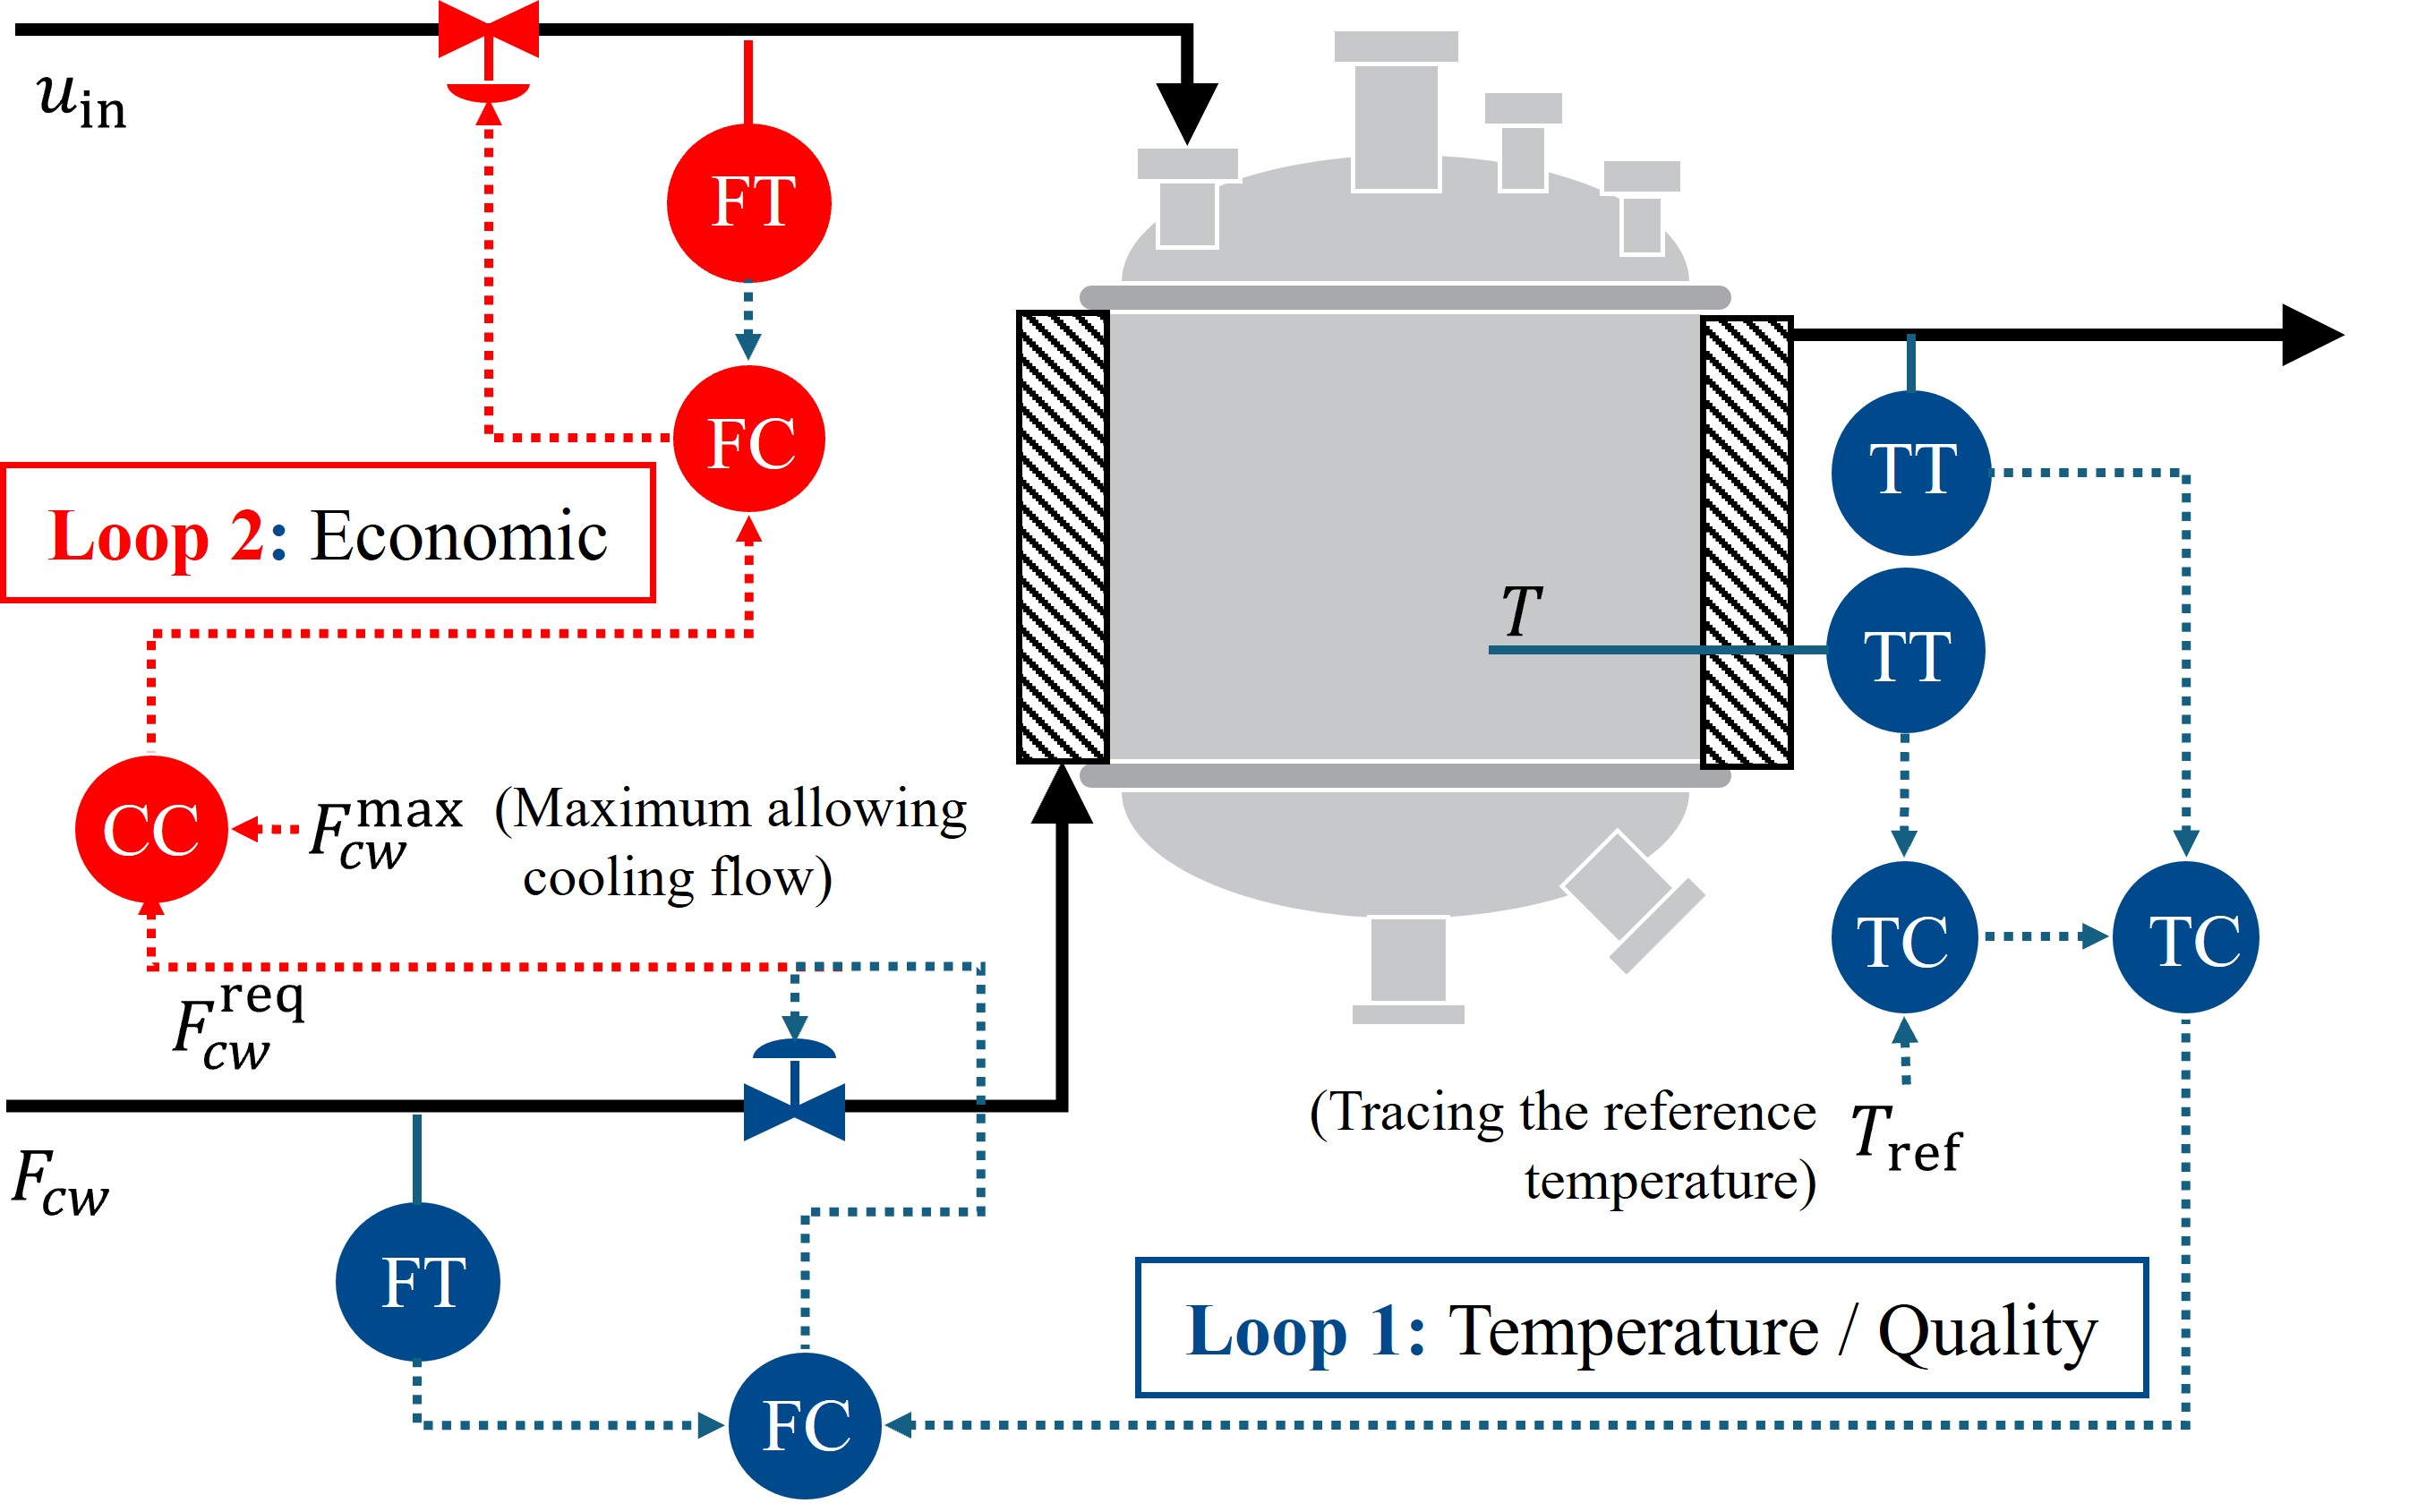
\includegraphics[width=16cm]{reactor_schematic.jpg}};
\begin{scope}[x={(art.south east)},y={(art.north west)}]
\fill[red] (.040,.432) rectangle (.087,.475);
\node[text=white,font=\fontsize{13}{15}\selectfont] at (.063,.452) {VPC};
\fill[white] (.005,.610) rectangle (.267,.682);
\node[text=red,align=center,font=\bfseries\fontsize{14}{16}\selectfont] at (.135,.646) {Economic VPC loop};
\fill[white] (.118,.390) rectangle (.416,.487);
\node[anchor=west,font=\fontsize{16}{18}\selectfont] at (.123,.451) {$F_{\mathrm{cw,sp}}$};
\node[align=center,font=\fontsize{11}{12}\selectfont] at (.308,.448) {(Cooling demand\\setpoint)};
\fill[white] (.061,.287) rectangle (.170,.356);
\node[anchor=west,font=\fontsize{17}{19}\selectfont] at (.065,.323) {$F_{\mathrm{cw}}^{\mathrm{v}}$};
\node[align=center,font=\fontsize{10}{11}\selectfont] at (.232,.315) {Virtual cooling\\demand};
\fill[white] (.530,.178) rectangle (.774,.287);
\node[align=center,font=\fontsize{11}{12}\selectfont] at (.638,.245) {Tracking the reference\\temperature};
\fill[white] (.765,.200) rectangle (.862,.272);
\node[font=\fontsize{17}{19}\selectfont] at (.808,.237) {$T_{\mathrm{ref}}$};
\fill[white] (.478,.083) rectangle (.886,.160);
\node[text=blue!50!black,align=center,font=\bfseries\fontsize{15}{17}\selectfont] at (.682,.120) {Temperature / quality loop};
\end{scope}
\end{tikzpicture}
\end{document}
